\section{جمع‌بندی و مسیر پیش‌رو}

% Slide 47
\begin{frame}{مسیر پیش‌رو: دروس مرتبط در دانشگاه مانهایم}{\lr{What's Next?}}
\begin{columns}[T,onlytextwidth]
\begin{column}{0.48\textwidth}
\begin{itemize}\small\setlength{\itemsep}{6pt}
    \item \textbf{پروفسور گملا}: \lr{(Prof.~Gemulla)}
    \begin{itemize}\footnotesize\setlength{\itemsep}{2pt}
        \item \textbf{نیم‌سال پاییز (\lr{HWS}):} کلان‌داده، یادگیری ماشین
        \item \textbf{نیم‌سال بهار (\lr{FSS}):} یادگیری عمیق \lr{(Deep Learning)}
    \end{itemize}
    \item \textbf{پروفسور بیزر}: \lr{(Prof.~Bizer)}
    \begin{itemize}\footnotesize\setlength{\itemsep}{2pt}
        \item \textbf{نیم‌سال پاییز (\lr{HWS}):} یکپارچه‌سازی وب، مدل‌های زبانی بزرگ
        \item \textbf{نیم‌سال بهار (\lr{FSS}):} وب‌کاوی \lr{(Web Mining)}
    \end{itemize}
    \item \textbf{پروفسور اشتوکن‌اشمیت}: \lr{(Prof.~Stuckenschmidt)}
    \begin{itemize}\footnotesize\setlength{\itemsep}{2pt}
        \item \textbf{نیم‌سال پاییز (\lr{HWS}):} سامانه‌های پشتیبان تصمیم‌گیری
    \end{itemize}
\end{itemize}
\end{column}%
\begin{column}{0.48\textwidth}
\begin{itemize}\small\setlength{\itemsep}{6pt}
    \item \textbf{پروفسور پونزتو}: \lr{(Prof.~Ponzetto)}
    \begin{itemize}\footnotesize\setlength{\itemsep}{2pt}
        \item \textbf{نیم‌سال پاییز (\lr{HWS}):} بازیابی اطلاعات و جستجوی وب
        \item \textbf{نیم‌سال بهار (\lr{FSS}):} تحلیل پیشرفتهٔ متن \lr{(Text Analytics)}
    \end{itemize}
    \item \textbf{پروفسور کویپر}: \lr{(Prof.~Keuper)}
    \begin{itemize}\footnotesize\setlength{\itemsep}{2pt}
        \item \textbf{نیم‌سال پاییز (\lr{HWS}):} بینایی ماشین پیشرفته
        \item \textbf{نیم‌سال بهار (\lr{FSS}):} مدل‌های مولد در بینایی ماشین
    \end{itemize}
    \item \textbf{پروفسور رهسه}: \lr{(Prof.~Rehse)}
    \begin{itemize}\footnotesize\setlength{\itemsep}{2pt}
        \item \textbf{نیم‌سال بهار (\lr{FSS}):} فرایندکاوی پیشرفته \lr{(Process Mining)}
    \end{itemize}
\end{itemize}
\end{column}
\end{columns}
\end{frame}

% Slide 48
\begin{frame}{پرسش و پاسخ}{\lr{Questions?}}
\begin{center}
\vspace{0.8cm}
{\huge\bfseries\color{mannheimblue} آیا سؤالی دارید؟}

\vspace{0.8cm}

\includegraphics[width=0.25\textwidth,keepaspectratio]{images/extracted_168.jpeg}
\end{center}
\end{frame}

% Slide 49
\begin{frame}{منابع درسی این بخش}{\lr{Literature for this Slideset}}
\begin{columns}[T,onlytextwidth]
\begin{column}{0.65\textwidth}
\begin{itemize}\setlength{\itemsep}{8pt}
    \item \textbf{کتاب مرجع اصلی:}
    \begin{latin}
    \small
    \textbf{Pang-Ning Tan, Michael Steinbach, Anuj Karpatne, Vipin Kumar}\\
    \textit{Introduction to Data Mining}, 2nd Edition. Pearson.
    \end{latin}
    \vspace{0.2cm}
    \item \textbf{فصل‌های مرتبط:}
    \begin{itemize}\setlength{\itemsep}{4pt}
        \item \textbf{فصل ۴:} تحلیل وابستگی: مفاهیم پایه و الگوریتم‌ها\\[2pt]
        {\footnotesize\lr{(Chapter 4: Basic Concepts and Algorithms)}}
        \item \textbf{فصل ۷:} تحلیل وابستگی: مفاهیم پیشرفته\\[2pt]
        {\footnotesize\lr{(Chapter 7: Advanced Concepts)}}
    \end{itemize}
\end{itemize}
\end{column}%
\begin{column}{0.32\textwidth}
\centering
\vspace{0.2cm}
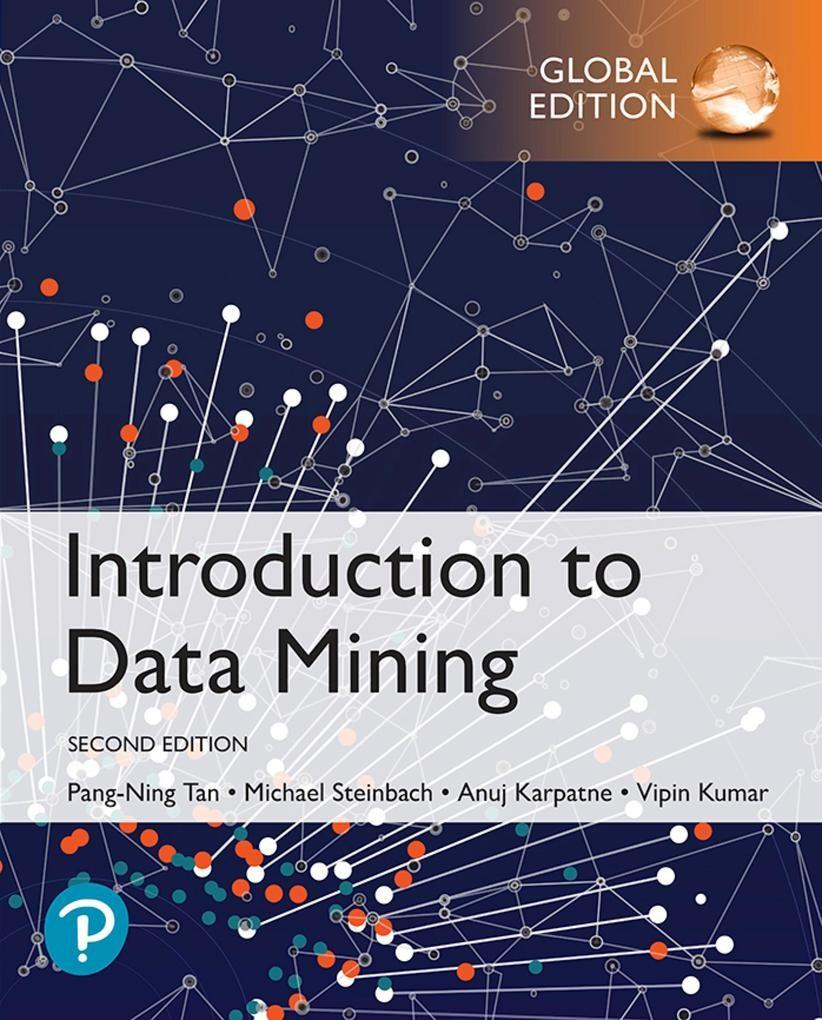
\includegraphics[width=0.85\textwidth,keepaspectratio]{images/extracted_171.jpeg}
\end{column}
\end{columns}
\end{frame}
